

\title{Investigative Physics\\ Module 1: Activity Units for Physics 131}


\author{E.F. Bunn,$^1$ M.S. Fetea,$^4$ G.P. Gilfoyle,$^1$ H. Nebel,$^1$ \\J. Singal,$^1$ M. Trawick,$^1$ P.D. Rubin,$^2$ and M.F. Vineyard$^3$\\[4pt]
$^1$Department of Physics, University of Richmond, VA 23173 \\[4pt]
$^2$Department of Physics, George Mason University, Fairfax, VA  22030 \\[4pt]
$^3$Department of Physics, Union College, Schenectady, NY 12308 \\[4pt]
$^4$Germanna Community College, Fredericksburg, VA 22408}

\maketitle
\begin{abstract}
The exercises in this manual have been developed to support an investigative
physics course that emphasizes active learning. Some of these units have been
taken from the Workshop Physics project at Dickinson College and the Tools for
Scientific Thinking project at Tufts University and modified for use at the
University of Richmond. Others have been developed locally.

The units are made up of activities designed to guide your investigations in
the laboratory. The written work will consist primarily of documenting your
class activities by filling in the entries in the spaces provided in the units.
The entries consist of observations, derivations, calculations, and answers
to questions. Although you may use the same data and graphs as your partner(s)
and discuss concepts with your classmates, all entries should reflect your own
understanding of the concepts and the meaning of the data and graphs you are
presenting. Thus, each entry should be written in your own words. Indeed, it
is very important to your success in this course that your entries reflect a
sound understanding of the phenomena you are observing and analyzing.

We wish to acknowledge the support we have received for this project from the
University of Richmond and the Instrumentation and Laboratory Improvement program of the National Science Foundation. Also, we would like to thank our laboratory directors for their invaluable technical assistance.
\end{abstract}

\begin{center}

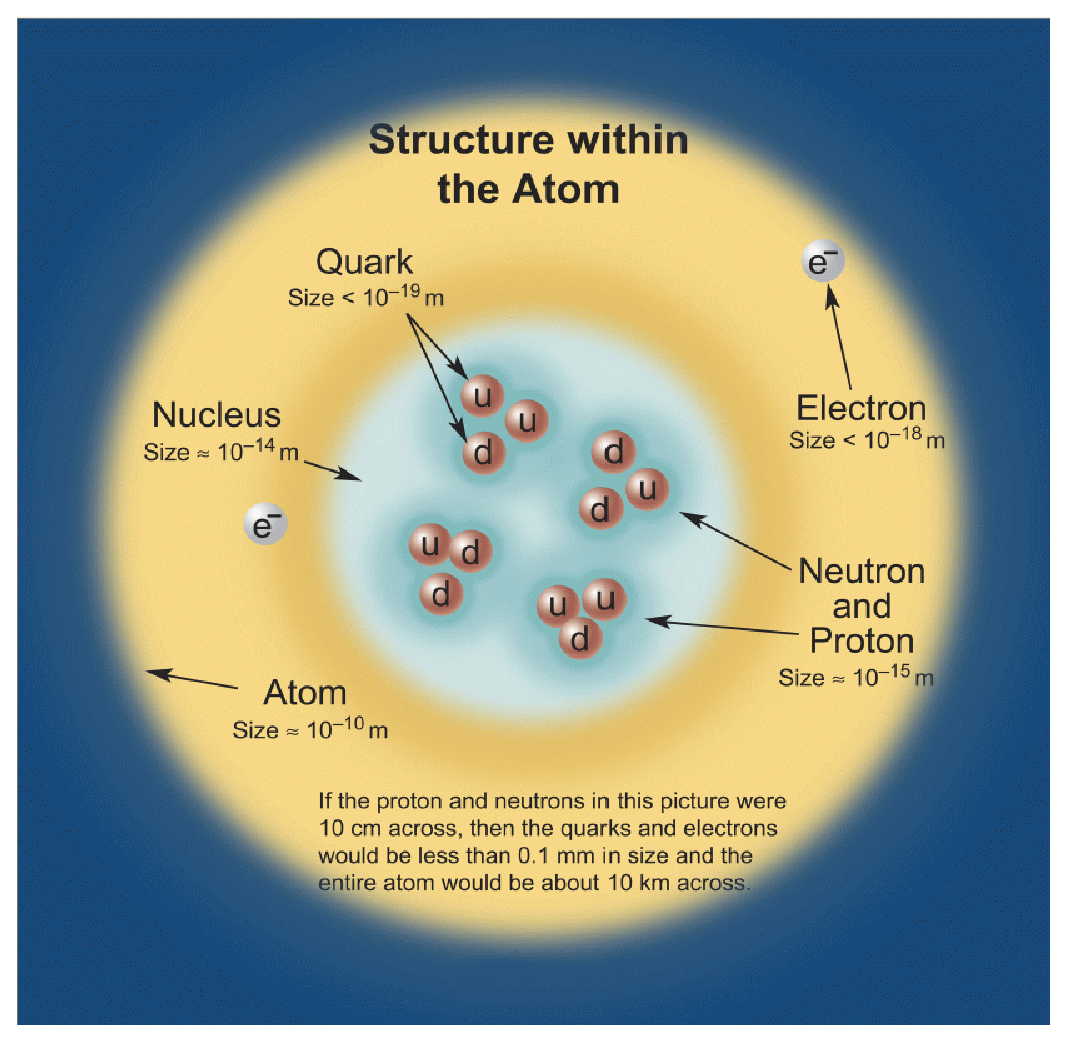
\includegraphics[width=3.2in]{AtomicStructure.ps}

\end{center}

\thispagestyle{empty}

\newpage


\ 
\setcounter{page}{2}

\vfill

Cover art: The atom consists of smaller electrons and a nucleus consisting of protons and neutrons. The protons and neutrons, in turn, are formed from objects called quarks and gluons. Courtesy, the American Institute of Physics.

\pagebreak
